\documentclass[11pt,a4paper]{jlreq}
\usepackage{amsmath}
\usepackage{amssymb}
\usepackage{empheq}
\usepackage[dvipdfmx]{graphicx}
\usepackage{booktabs}
\usepackage{listings}
\usepackage{float}

\begin{document}

\begin{center}
{\LARGE \textbf{情報科学基礎A 第8回 レポート}}
\end{center}
\vspace{1em}

\begin{flushright}
提出日：\today \\
学籍番号：2611193 \\
氏名：中井平蔵
\end{flushright}

\section*{Task 1：解析解}

\subsection*{(1) \boldmath$\ddot{x}+3\dot{x}+x=0$\unboldmath の場合}
初めに、解を $x(t)=e^{\lambda t}$ と仮定すると、特性方程式は以下のようになる。
\[
\lambda^2+3\lambda+1=0
\]

よって固有値は、

\[
\lambda_{1,2}=\frac{-3\pm\sqrt{5}}{2}
\]

となる。したがって、一般解は以下のようになる。
\[
x(t)=C_1 e^{\textstyle \frac{-3+\sqrt{5}}{2}t}+C_2 e^{\textstyle \frac{-3-\sqrt{5}}{2}t}
\]

次に初期条件を用いて定数 $C_1,C_2$ を求める。
\[
x(0)=1 \;\Rightarrow\; C_1+C_2=1
\]

また、$x(t)$を微分すると、
\[
\dot{x}(t)=\frac{-3+\sqrt{5}}{2}C_1 e^{\textstyle \frac{-3+\sqrt{5}}{2}t}
+\frac{-3-\sqrt{5}}{2}C_2 e^{\textstyle \frac{-3-\sqrt{5}}{2}t}
\]

より、

\[
\dot{x}(0)=0 \;\Rightarrow\; \dot{x}(0)=\frac{-3+\sqrt{5}}{2}C_1+\frac{-3-\sqrt{5}}{2}C_2=0
\]

したがって、以下の連立方程式を求めることで $C_1,C_2$ を得る。
\begin{subequations}
\begin{empheq}[left={\empheqlbrace\,}, right={}]{align}
&C_1+C_2=1\\
&\dfrac{-3+\sqrt{5}}{2}C_1+\dfrac{-3-\sqrt{5}}{2}C_2=0
\end{empheq}
\end{subequations}

$(1a)$の式から$C_2=1-C_1$が得られるので、これを$(1b)$の式に代入すると、

\[
\frac{-3+\sqrt{5}}{2}C_1+\frac{-3-\sqrt{5}}{2}(1-C_1)=0
\]
\[
\;\Rightarrow\;
\frac{-3+\sqrt{5}}{2}C_1+\frac{-3-\sqrt{5}}{2}-\frac{-3-\sqrt{5}}{2}C_1=0
\]
\[
\;\Rightarrow\;
\left(\frac{-3+\sqrt{5}}{2}-\frac{-3-\sqrt{5}}{2}\right)C_1=-\frac{-3-\sqrt{5}}{2}
\]
\[
\;\Rightarrow\;
\sqrt{5}\,C_1=\frac{3+\sqrt{5}}{2}
\]
\[
C_1=\frac{3+\sqrt{5}}{2\sqrt{5}}=\frac{5+3\sqrt{5}}{10}
\]

よって、
\[
C_2=1-C_1=1-\frac{5+3\sqrt{5}}{10}=\frac{5-3\sqrt{5}}{10}
\]

となるため、
\[
C_1=\frac{5+3\sqrt{5}}{10},\qquad C_2=\frac{5-3\sqrt{5}}{10}
\]

が得られる。したがって、解析解は以下のようになる。
\[
\boxed{
x(t)=\frac{5+3\sqrt{5}}{10}e^{\textstyle \frac{-3+\sqrt{5}}{2}t}
+\frac{5-3\sqrt{5}}{10}e^{\textstyle \frac{-3-\sqrt{5}}{2}t}
}
\]


\subsection*{(2) \boldmath$\ddot{x}+1001\dot{x}+1000x=0$\unboldmath の場合}
同様に特性方程式は
\[
\lambda^2+1001\lambda+1000=0
\]

であり、因数分解すると
\[
(\lambda+1)(\lambda+1000)=0
\]

となる。したがって固有値は
\[
\lambda_1=-1,\qquad \lambda_2=-1000
\]

である。したがって、一般解は以下のようになる。
\[
x(t)=C_1 e^{-t}+C_2 e^{-1000t}
\]

次に初期条件を用いて定数 $C_1,C_2$ を求める。
\[
C_1+C_2=1
\]

また、$x(t)$を微分すると、
\[
\dot{x}(t)=-C_1 e^{-t}-1000C_2 e^{-1000t}
\]

より、
\[
\dot{x}(0)=-C_1-1000C_2=0
\]

したがって、以下の連立方程式を求めることで $C_1,C_2$ を得る。
\begin{subequations}
\begin{empheq}[left={\empheqlbrace\,}, right={}]{align}
&C_1+C_2=1\\
&C_1+1000C_2=0
\end{empheq}
\end{subequations}

$(2a)$の式から$C_1=1-C_2$が得られるので、これを$(2b)$の式に代入すると、
\[
1-C_2+1000C_2=0
\]
\[
\;\Rightarrow\;
999C_2=-1
\]
\[
\;\Rightarrow\;
C_2=-\frac{1}{999}
\]

よって、
\[
C_1=1-C_2=1+\frac{1}{999}=\frac{1000}{999}
\]

となるため、
\[
C_1=\frac{1000}{999},\qquad C_2=-\frac{1}{999}
\]

が得られる。したがって、解析解は以下のようになる。
\[
\boxed{
x(t)=\frac{1000}{999}e^{-t}-\frac{1}{999}e^{-1000t}
}
\]

\section*{Task 2：状態空間表現}

Task 1 の2階微分方程式を、連立1階微分方程式に書き換える。

\[
\mathbf{y}=\begin{bmatrix}y_1\\y_2\end{bmatrix}
=\begin{bmatrix}x\\\dot{x}\end{bmatrix}
\]

とおく。このとき以下が成り立つ。
\[
\dot{y}_1=y_2
\]

\subsection*{(1) 系 \boldmath$\ddot{x}+3\dot{x}+x=0$\unboldmath}
元の方程式を $\ddot{x}$ について解くと
\[
\ddot{x}=-3\dot{x}-x
\]

であるため、
\[
\dot{y}_2=-3y_2-y_1
\]

となる。したがって、
\[
\boxed{
\begin{bmatrix}\dot{y}_1\\\dot{y}_2\end{bmatrix}
=
\begin{bmatrix}0&1\\-1&-3\end{bmatrix}
\begin{bmatrix}y_1\\y_2\end{bmatrix}
}
\]

となる。

\subsection*{(2) 系 \boldmath$\ddot{x}+1001\dot{x}+1000x=0$\unboldmath}
同様に、
\[
\ddot{x}=-1001\dot{x}-1000x
\]

であるため、
\[
\dot{y}_2=-1001y_2-1000y_1
\]

となる。したがって、
\[
\boxed{
\begin{bmatrix}\dot{y}_1\\\dot{y}_2\end{bmatrix}
=
\begin{bmatrix}0&1\\-1000&-1001\end{bmatrix}
\begin{bmatrix}y_1\\y_2\end{bmatrix}
}
\]

となる。

\section*{Task 3：オイラー法による数値解}

Task 2 で得た状態空間表現
\[
\dot{\mathbf{y}}=A\mathbf{y},\qquad
\mathbf{y}=\begin{bmatrix}x\\ \dot{x}\end{bmatrix}
\]

に対して、時刻を $t_n=nh$（$n=0,1,2,\dots,N$）とおく。まず微分方程式
\[
\dot{\mathbf{y}}=A\mathbf{y}
\]

の左辺を前進差分で近似すると、
\[
\dot{\mathbf{y}}(t_n)\approx\frac{\mathbf{y}_{n+1}-\mathbf{y}_n}{h}
\]

となる。これを代入して整理すると、
\[
\mathbf{y}_{n+1}=\mathbf{y}_n+hA\mathbf{y}_n
\]

を得る。

具体的には、$\mathbf{y}_n=\begin{bmatrix}x_n\\ \dot{x}_n\end{bmatrix}$ として次のように計算する。
\begin{itemize}
\item[(i)] 系(1): \ $\ddot{x}+3\dot{x}+x=0$
\[
\begin{bmatrix}x_{n+1}\\ \dot{x}_{n+1}\end{bmatrix}
=
\begin{bmatrix}x_n\\ \dot{x}_n\end{bmatrix}
+
h
\begin{bmatrix}0&1\\-1&-3\end{bmatrix}
\begin{bmatrix}x_n\\ \dot{x}_n\end{bmatrix}
\]
\[
\Longrightarrow\quad
\left\{
\begin{aligned}
x_{n+1}&=x_n+h\,\dot{x}_n\\
\dot{x}_{n+1}&=\dot{x}_n+h(-x_n-3\dot{x}_n)
\end{aligned}
\right.
\]
\item[(ii)] 系(2): \ $\ddot{x}+1001\dot{x}+1000x=0$
\[
\begin{bmatrix}x_{n+1}\\ \dot{x}_{n+1}\end{bmatrix}
=
\begin{bmatrix}x_n\\ \dot{x}_n\end{bmatrix}
+
h
\begin{bmatrix}0&1\\-1000&-1001\end{bmatrix}
\begin{bmatrix}x_n\\ \dot{x}_n\end{bmatrix}
\]
\[
\Longrightarrow\quad
\left\{
\begin{aligned}
x_{n+1}&=x_n+h\,\dot{x}_n\\
\dot{x}_{n+1}&=\dot{x}_n+h(-1000x_n-1001\dot{x}_n)
\end{aligned}
\right.
\]
\end{itemize}

初期値は、
\[
x_0=1,\qquad \dot{x}_0=0
\]

である。計算区間は $0\le t\le 3$ とし、刻み幅は
\[
h\in\{0.5,\ 0.2,\ 0.1,\ 0.05,\ 0.01,\ 0.002,\ 0.001\}
\]

とした。各 $h$ について $N=3/h$ ステップ計算し、得られた $x_n$ を数値解 $x_h(t_n)$ として比較に用いた。

\section*{Task 4：解析解との比較}

各刻み幅 $h$ について、数値解 $x_h(t)$ と解析解 $x(t)$ の最大絶対誤差
\[
E_\infty=\max_{0\le n\le N}|x_h(t_n)-x(t_n)|
\]

を計算した。結果を表に示す。
\vspace{0.8em}
\begin{table}[H]
\centering
\caption{刻み幅 $h$ に対する最大絶対誤差 $E_\infty$ の比較}
\vspace{0.3em}
\begin{tabular*}{0.9\textwidth}{@{\extracolsep{\fill}}ccc@{}}
\toprule
$h$ & 系(1) の最大誤差 $E_\infty$ & 系(2) の最大誤差 $E_\infty$ \\
\midrule
0.5   & 7.887e-02 & 1.545e+13 \\
0.2   & 1.683e-02 & 3.043e+31 \\
0.1   & 8.257e-03 & 7.404e+56 \\
0.05  & 4.089e-03 & 2.583e+98 \\
0.01  & 8.116e-04 & 1.876e+283 \\
0.002 & 1.621e-04 & 1.370e-03 \\
0.001 & 8.102e-05 & 3.677e-04 \\
\bottomrule
\end{tabular*}
\end{table}
\vspace{0.8em}
表より、系(1)では $h$ を小さくすると単調に誤差が減少し、前進オイラー法が収束していることが分かる。
一方で系(2)では、$h=0.01$ 以上で誤差が極端に大きくなり不安定となるが、$h=0.002,\ 0.001$ では誤差が小さくなる。
これは、系(2)の固有値に対する前進オイラー法の安定条件が厳しいためである。

比較図を以下に示す。

\begin{figure}[H]
\centering
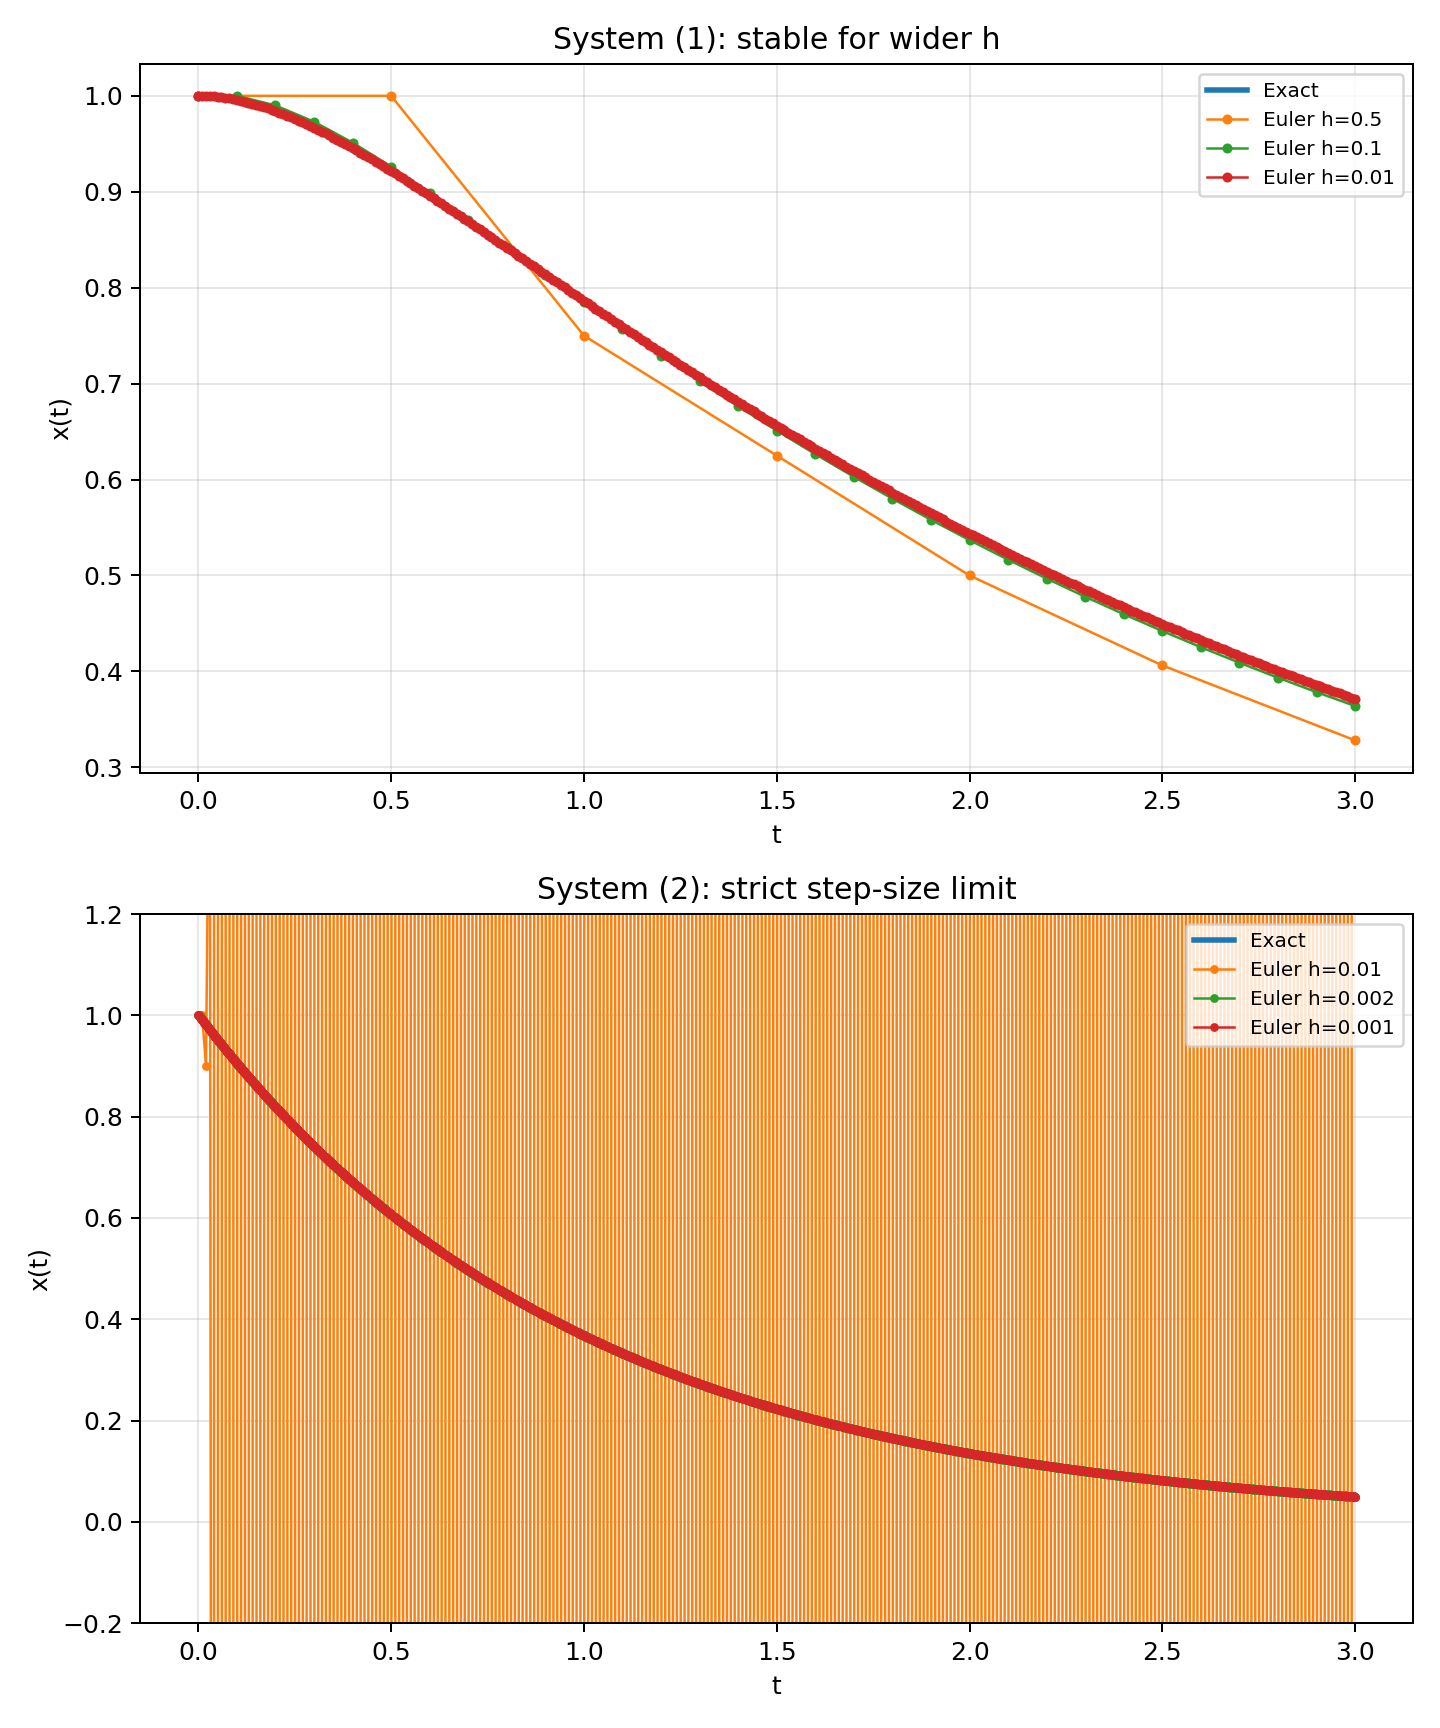
\includegraphics[width=\linewidth]{img/task34_compare.png}
\caption{オイラー法による数値解と解析解の比較（上：系(1)、下：系(2)）}
\end{figure}

\section*{Task 5：刻み幅 $h$ が安定性・精度に与える影響}

安定条件を説明するために、1次の線形方程式
\[
\dot{x}=\lambda x
\]

を考える。これに前進オイラー法を適用すると、
\[
x_{n+1}=x_n+h\lambda x_n=(1+h\lambda)x_n
\]

となる。よって、
\[
x_n=(1+h\lambda)^n x_0
\]

したがって、$n\to\infty$ で解が発散しないためには、以下の条件が求められる。
\[
|1+h\lambda|<1
\]

一般には $\lambda$ は正・負・複素数を取り得るが、ここでは今回の対象系の固有値がすべて負の実数であることに対応して、$\lambda<0$ の場合に限定して条件を展開する。
\[
|1+h\lambda|<1
\]
\[
\Rightarrow\;
-1<1+h\lambda<1
\]
\[
\Rightarrow\;
-2<h\lambda<0
\]

ここで $\lambda<0$であるため、$\lambda$ で割ると不等号の向きが反転して、
\[
\frac{-2}{\lambda}>h>0
\]

となる。さらに $|\lambda|=-\lambda$ を用いると
\[
0<h<\frac{2}{|\lambda|}
\]

を得る。

この条件から、刻み幅 $h$ を大きくすると$|1+h\lambda|$ が $1$ を超えやすくなり、不安定化しやすいことが分かる。
一方で、$h$ を小さくすると安定し、Task 4 の誤差表でもわかる通り、実際に誤差は減少する。
さらに精度については、前進オイラー法の1ステップ局所離散化誤差が
\[
\tau_n=O(h^2)
\]
であり、$T=Nh$ を固定した区間での大域誤差は
\[
\max_{0\le n\le N}|x(t_n)-x_n|=O(h)
\]
となる。したがって、$h$ を小さくするほど大域誤差は一次的に減少し、精度が向上する。
すなわち、$h$ が大きいほど不安定になりやすく、$h$ が小さいほど安定し、精度は高くなるが計算コストは増える。

\section*{Task 6：2つの系の数値挙動の違い}

具体的に各系での収束する$h$の範囲を考える。

系(2)の固有値は、
\[
\lambda_1=-1,\qquad \lambda_2=-1000
\]

であり、Task 5 で示した安定条件
\[
0<h<\frac{2}{|\lambda|}
\]

を各固有値に適用すると、
\[
\lambda_1=-1\;\Rightarrow\; 0<h<2,
\]
\[
\lambda_2=-1000\;\Rightarrow\; 0<h<0.002
\]

となる。よって、収束する$h$の範囲は以下のようになる。
\[
0<h<0.002
\]

このため、例えば $h=0.01$ では、
\[
|1-1000h|=|1-10|=9>1
\]

となり $1$ を超えるため、不安定化して誤差が急激に増大する。

一方、系(1)の固有値は
\[
\lambda_1=\frac{-3+\sqrt{5}}{2},\qquad \lambda_2=\frac{-3-\sqrt{5}}{2}
\]

であり、Task 5 で示した安定条件
\[
0<h<\frac{2}{|\lambda|}
\]

を各固有値に適用すると、
\[
\lambda_1=\frac{-3+\sqrt{5}}{2}\;\Rightarrow\; 0<h<\frac{2}{(3-\sqrt{5})/2}=3+\sqrt{5},
\]
\[
\lambda_2=\frac{-3-\sqrt{5}}{2}\;\Rightarrow\; 0<h<\frac{2}{(3+\sqrt{5})/2}=3-\sqrt{5}
\]

となる。よって、収束する$h$の範囲は以下のようになる。
\[
0<h<3-\sqrt{5}\approx 0.764
\]

以上より、2つの系の数値挙動の違いは次のように要約できる。  
系(1)は安定に計算できる刻み幅の範囲が比較的広く（$0<h<3-\sqrt{5}\approx0.764$）、刻み幅をある程度大きくしても計算が破綻しにくい。  
これに対して系(2)は安定条件が $0<h<0.002$ と非常に厳しく、わずかに刻み幅を大きくすると誤差が急激に増大して不安定化する。  
したがって、同じ前進オイラー法でも、系(1)は扱いやすく、系(2)は非常に小さい刻み幅を要求するという点が本質的な違いである。

\clearpage
\section*{付録：Task 3・4 検証用Pythonコード}
\lstset{basicstyle=\ttfamily\small,breaklines=true,frame=single}
\lstinputlisting{scripts/task34_euler.py}

\end{document}
